\chapter{System Architecture and Design}

\section{Introduction}

This chapter presents the overall architecture and design of the proposed intelligent carpooling platform. It focuses on the structural organization of the system, the interactions between its components, and the key design decisions that guided its conception.

The objective of this chapter is to provide a comprehensive understanding of how the system is structured prior to implementation. It includes a global architectural overview, a detailed description of system components, and modeling through use case and class diagrams. Additionally, the data flow within the system is analyzed to illustrate how information is processed and exchanged.

\section{Global System Architecture}
The architectural foundation of the system was established during \textbf{Sprint 0}, which focused on project initialization, environment setup, and the definition of the global system structure. This initial phase enabled the identification of core components and their interactions, forming the basis for subsequent development.

The proposed system follows a layered architecture composed of three main components: the frontend, the backend, and the data layer.
The proposed system follows a layered architecture composed of three main components: the frontend, the backend, and the data layer. This separation ensures modularity, scalability, and maintainability.

\begin{itemize}
    \item \textbf{Frontend Layer:} A mobile application developed using Flutter, responsible for user interaction and interface rendering.
    \item \textbf{Backend Layer:} A server implemented using Flask, acting as the core processing layer of the system. It handles business logic, intelligent matching, and data processing.
    \item \textbf{Data Layer:} A PostgreSQL database used to store and manage system data efficiently.
\end{itemize}

The interaction between these components is illustrated in Figure~\ref{fig:global_architecture}.

\begin{figure}[htbp]
    \centering
    \includegraphics[width=0.85\textwidth]{images/architecture/global_architecture.png}
    \caption{Global System Architecture}
    \label{fig:global_architecture}
\end{figure}

The mobile application serves as the entry point for user interactions, sending HTTP requests to the backend through RESTful APIs and receiving structured JSON responses. Real-time communication is ensured through WebSocket connections, enabling instant updates such as notifications and ride status changes.

The backend represents the core processing layer of the system. It integrates multiple responsibilities, including request handling, business logic execution, geospatial processing, and intelligent decision-making. This centralized design ensures consistency and efficient coordination between system components.

The backend interacts with the PostgreSQL database through SQL queries to store and retrieve persistent data. Additionally, it communicates with external geospatial services, specifically OSRM, to obtain routing and distance information required for ride matching.

This architecture ensures a clear separation of concerns while maintaining efficient communication between components, supporting scalability and modular system evolution.

\begin{table}[H]
\centering
\begin{tabular}{|l|l|l|}
\hline
\textbf{Component} & \textbf{Technology} & \textbf{Role} \\
\hline
Frontend & Flutter & User interface and interaction \\
Backend & Flask & Business logic and API management \\
Database & PostgreSQL & Data storage and management \\
External Services & OSRM / OSM & Route computation and geospatial data \\
\hline
\end{tabular}
\caption{System Components Overview}
\end{table}

\section{Architectural Design Decisions}

Several design decisions were made to ensure that the system meets both functional and non-functional requirements.

\subsection{Layered Architecture}

A layered architecture was adopted to separate concerns between the user interface, business logic, and data management. This approach improves maintainability and allows independent evolution of system components.

\subsection{Client-Server Model}

The system follows a client-server architecture, where the frontend communicates with the backend through RESTful APIs. This design enables scalability and supports multiple clients.

\subsection{Technology Selection Rationale}

The choice of technologies was driven by system requirements. Flask provides flexibility for backend logic, Flutter enables cross-platform mobile development, and PostgreSQL ensures reliable and efficient data management.

\subsection{Architectural Trade-offs and Design Justification}

The architectural choices presented in this chapter were not merely technological selections but deliberate engineering decisions grounded in the project scope, operational constraints, and long-term maintainability requirements. This subsection provides a rigorous justification of the four foundational design decisions that shaped the system.

\subsubsection{Monolithic Architecture over Microservices}

A modular monolithic architecture was chosen over a distributed microservices approach. While microservices offer independent scalability and deployment autonomy, they introduce significant operational overhead in terms of service orchestration, inter-service communication, and consistency management. Given the project's scope---a single enterprise application with a controlled user base---the operational complexity of microservices would outweigh their benefits.

The monolithic approach, structured around clearly separated internal modules (authentication, ride management, matching, real-time communication, and prediction), preserves development simplicity while maintaining logical modularity. This design reduces deployment overhead, simplifies debugging, and ensures transactional consistency across domain boundaries without requiring distributed coordination protocols.

\subsubsection{Backend-Centric Business Logic Enforcement}

All business logic is centralized in the backend layer, with the frontend functioning exclusively as a presentation and interaction layer. This decision was driven by three primary considerations.

First, consistency: by enforcing all rules server-side, the system guarantees uniform behavior regardless of the client platform or version. Second, security: business rules cannot be circumvented through client-side manipulation, which is particularly critical for ride booking constraints, authentication, and administrative operations. Third, evolvability: modifying a business rule requires a single backend change rather than coordinating updates across multiple client implementations.

This backend-centric model ensures that the frontend remains stateless and thin, reducing client complexity while strengthening the system's integrity.

\subsubsection{REST and WebSocket Hybrid Communication}

The system employs a hybrid communication model combining RESTful APIs with WebSocket connections. REST is used for all stateless request-response operations such as authentication, profile updates, ride creation, and search queries. WebSocket is reserved exclusively for real-time, event-driven updates.

This separation is intentional. Polling-based approaches, while simpler to implement, introduce unnecessary network overhead and latency, particularly for high-frequency updates such as ride status transitions and location tracking. WebSocket provides persistent bidirectional channels that allow the backend to push updates asynchronously, eliminating redundant client requests while ensuring immediate state synchronization across all connected participants.

The hybrid model thus optimizes resource usage: REST handles transactional operations efficiently, while WebSocket guarantees low-latency propagation of state changes.

\subsubsection{Centralized Geospatial Processing}

All geospatial computations, including route analysis, corridor construction, and detour estimation, are executed server-side through the OSRM integration. This centralization ensures that matching logic remains consistent and cannot be influenced by client-side approximations or device-specific positioning inaccuracies.

Furthermore, by keeping geospatial intelligence in the backend, the system maintains control over algorithmic evolution. Improvements to matching strategies, scoring criteria, or corridor parameters can be deployed without requiring client updates. This design also protects proprietary matching logic from inspection and reduces the computational burden on mobile devices.

\section{System Components Description}

\subsection{Frontend Layer}

The frontend is implemented as a mobile application using Flutter. It provides an intuitive user interface and manages all user interactions, including ride creation, ride search, booking, and notifications.

The frontend communicates with the backend through HTTP requests and maintains real-time synchronization using WebSocket connections.

\subsection{Backend Layer}

The backend serves as the central processing unit of the system. It is responsible for handling incoming requests, executing business logic, and coordinating communication between system components.

It integrates several functional modules, including:
\begin{itemize}
    \item REST API for client communication
    \item Business logic layer
    \item Geospatial matching engine
    \item Machine learning prediction module
\end{itemize}

\subsection{Data Layer}

The data layer is implemented using PostgreSQL. It manages persistent data storage, including users, rides, reservations, and system interactions.

The database ensures data integrity, consistency, and efficient querying. It supports structured data organization and enforces relational constraints between entities, ensuring reliable management of system data.

Additionally, PostgreSQL provides advanced features such as indexing and optimized query execution, which improve performance when handling large volumes of data.

\section{Global Use Case Diagram}

The global use case diagram represents the interactions between users and the system.

\begin{figure}[H]
    \centering
    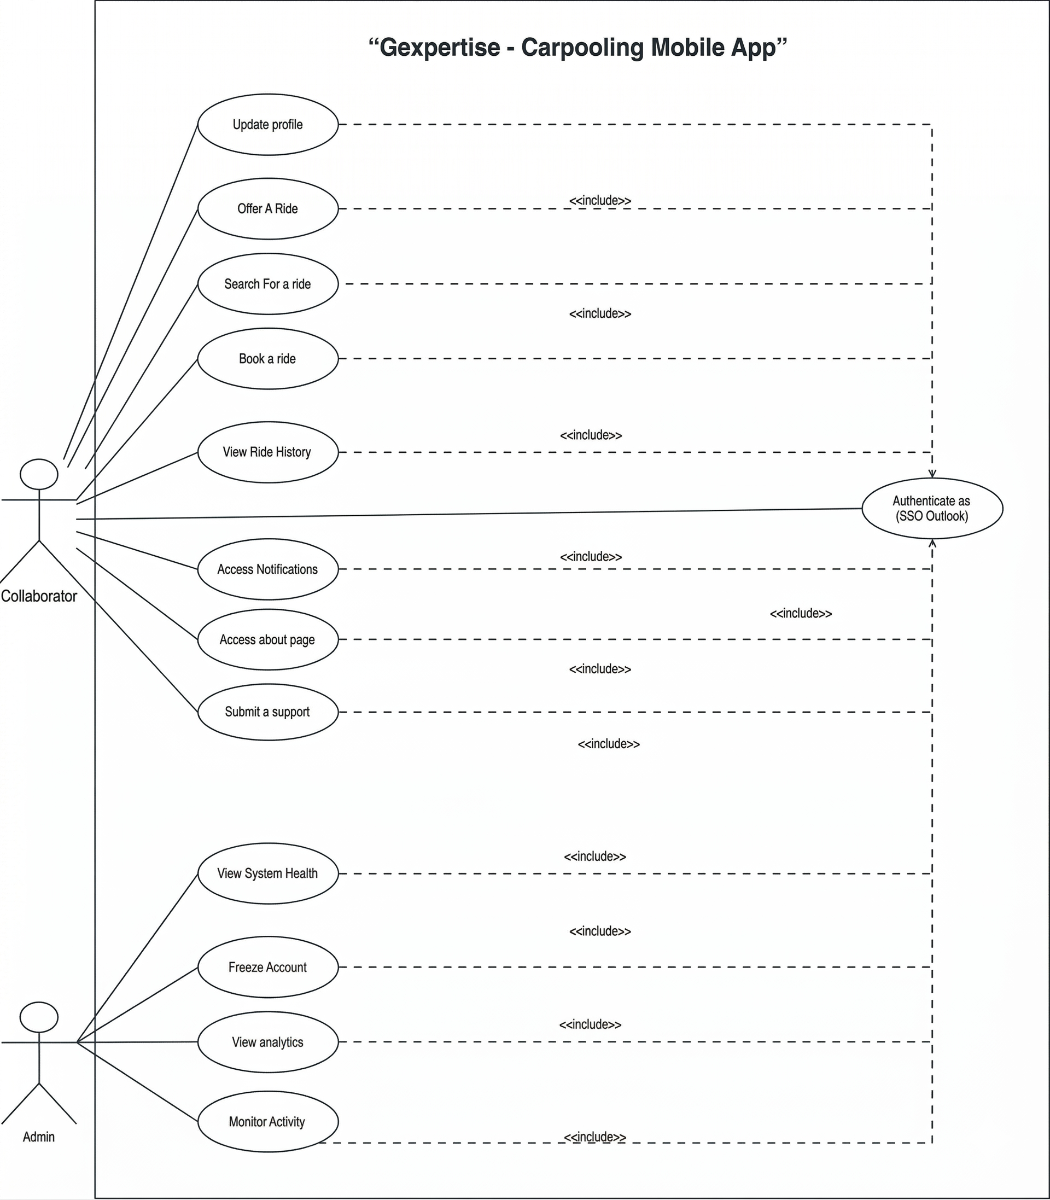
\includegraphics[width=0.7\textwidth]{images/diagrams/use_case_global.png}
    \caption{Global Use Case Diagram}
    \label{fig:use_case}
\end{figure}

Two primary actors are identified: the collaborator and the administrator.

The collaborator can perform operations such as offering a ride, searching for rides, booking rides, managing their profile, and accessing notifications.

The administrator is responsible for system supervision tasks, including monitoring activity, managing user accounts, and ensuring system integrity.

Most functionalities require prior authentication, modeled through inclusion relationships with the authentication use case.

\section{Global Class Diagram}

The global class diagram presents the main entities of the system and their relationships.

\begin{figure}[H]
    \centering
    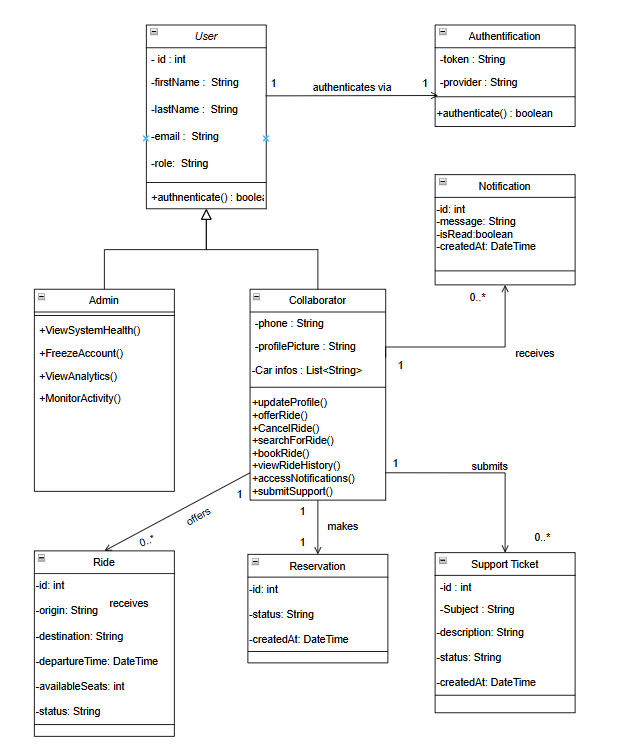
\includegraphics[width=0.7\textwidth]{images/diagrams/class_global.png}
    \caption{Global Class Diagram}
    \label{fig:class_diagram}
\end{figure}

The central entity is the User class, which is specialized into Collaborator and Admin roles.

The Collaborator interacts with core entities such as Ride, Reservation, Notification, and Support Ticket.

The Ride entity represents a carpooling offer, while the Reservation entity models booking operations.

This structure promotes modularity and extensibility, allowing the system to evolve without disrupting existing components.

\section{Data Flow Description}

A typical system interaction scenario is described as follows:

\begin{enumerate}
    \item A collaborator initiates an action via the mobile application.
    \item The frontend sends an HTTP request to the backend.
    \item The backend processes the request using business logic and matching logic.
    \item The backend queries the PostgreSQL database if necessary.
    \item The backend interacts with OSRM for geospatial computations.
    \item The processed result is returned as a JSON response.
    \item The frontend updates the interface accordingly.
    \item Real-time updates are transmitted through WebSocket connections.
\end{enumerate}

\section{Integration of Intelligent Components}

The system integrates two complementary intelligent approaches.

The first is a deterministic matching system based on geospatial analysis, which identifies optimal ride matches using real-time data.

The second is a machine learning module designed to analyze historical (or synthetic) data to predict commuting patterns and suggest future ride opportunities.

These components are integrated into the backend while maintaining modular separation. Their detailed implementation is presented in Chapter~5.

\section{Communication and Security}

Communication between system components is achieved through RESTful APIs and WebSocket protocols.

Security is ensured through authentication mechanisms, access control, and secure data exchange, guaranteeing that only authorized users can access system functionalities.

\section{Scalability and Maintainability Considerations}

The architecture was designed with scalability and maintainability in mind.

The separation of layers allows independent evolution of system components. The use of APIs enables integration with additional clients, and the modular backend design facilitates future enhancements.

\section{System Constraints}

The system operates under several constraints that influenced its design:

\begin{itemize}
    \item Dependency on external geospatial services (OSRM)
    \item Network latency affecting real-time communication
    \item Mobile device limitations such as battery consumption and connectivity variability
    \item Limited availability of real-world historical data for machine learning training
\end{itemize}

\section{Conclusion}

This chapter presented the architecture and design of the intelligent carpooling system, including its layered structure, component interactions, and system modeling.

The proposed architecture provides a robust and scalable foundation for implementing the platform’s functionalities.

The next chapter focuses on the implementation of user management and authentication features.